\documentclass{article}
%%
%% Default settings for artisynth
%%
\NeedsTeXFormat{LaTeX2e}
%%\ProvidesPackage{artisynthDoc}[2012/04/05]

\usepackage[T1]{fontenc}
\usepackage[latin1]{inputenc}
\usepackage{listings}
\usepackage{makeidx}
\usepackage{latexml}
\usepackage{graphicx}
\usepackage{framed}
\usepackage{booktabs}
\usepackage{color}

\newcommand{\pubdate}{\today}
\newcommand{\setpubdate}[1]{\renewcommand{\pubdate}{#1}}
\newcommand{\code}[1]{{\tt #1}}

\iflatexml
\usepackage{hyperref}
\setlength\parindent{0pt} 
\else
%% then we are making a PDF, so include things that LaTeXML can't handle: 
%% docbook style, \RaggedRight
\usepackage{ifxetex}
\usepackage{xstring}
\usepackage{pslatex} % fixes fonts; in particular sets a better-fitting \tt font

\usepackage[most]{tcolorbox}
\definecolor{shadecolor}{rgb}{0.95,0.95,0.95}
\tcbset{
    frame code={}
    center title,
    left=0pt,
    right=0pt,
    top=0pt,
    bottom=0pt,
    colback=shadecolor,
    colframe=white,
    width=\dimexpr\textwidth\relax,
    enlarge left by=0mm,
    boxsep=0pt,
    arc=0pt,outer arc=0pt,
}%

\usepackage[A4]{artisynth_papersize}
%\usepackage[letter]{artisynth_papersize}
\usepackage[hyperlink]{asciidoc-dblatex} 

%\usepackage{verbatim}
\usepackage{ragged2e}
\setlength{\RaggedRightRightskip}{0pt plus 4em}
\RaggedRight
\renewcommand{\DBKpubdate}{\pubdate}
\renewcommand{\DBKreleaseinfo}{}
\fi

% set hypertext links to be dark blue:
\definecolor{darkblue}{rgb}{0,0,0.8}
\definecolor{sidebar}{rgb}{0.5,0.5,0.7}
\hypersetup{colorlinks=true,urlcolor=darkblue,linkcolor=darkblue,breaklinks=true}

%%%%%%%%%%%%%%%%%%%%%%%%%%%%%%%%%%%%%%%%%%%%%%%%%%%%%%%%%%%%%%%%%%%%%%%%%%%%%
%
% Define macros for handling javadoc class and method references
%
%%%%%%%%%%%%%%%%%%%%%%%%%%%%%%%%%%%%%%%%%%%%%%%%%%%%%%%%%%%%%%%%%%%%%%%%%%%%%
\makeatletter

% macro to enable line break if inside a PDF file
\def\pdfbreak{\iflatexml\else\\\fi}

% code inspired by http://stackoverflow.com/questions/2457780/latex-apply-an-operation-to-every-character-in-a-string
\def\removeargs #1{\doremoveargs#1$\wholeString\unskip}
\def\doremoveargs#1#2\wholeString{\if#1$%
\else\if#1({()}\else{#1}\taketherest#2\fi\fi}
\def\taketherest#1\fi
{\fi \doremoveargs#1\wholeString}

% Note: still doesn't work properly when called on macro output ...
% i.e., \dottoslash{\concatnames{model}{base}{foo}} fails 
\def\dottoslash #1{\dodottoslash#1$\wholeString\unskip}
\def\dodottoslash#1#2\wholeString{\if#1$%
\else\if#1.{/}\else{#1}\fi\dottaketherest#2\fi}
\def\dottaketherest#1\fi{\fi \dodottoslash#1\wholeString}

\def\hashtodot #1{\dohashtodot#1$\wholeString\unskip}
\def\dohashtodot#1#2\wholeString{\if#1$X%
\else\if#1\#{.}\else{#1}\fi\hashtaketherest#2\fi}
\def\hashtaketherest#1\fi{\fi \dohashtodot#1\wholeString}

%\dollartodot{#1} does the same thing as \StrSubstitute[0]{#1}{\$}{.}
% from the packahe xstring. We define \dollartodot instead because
% LaTeXML does not implement xstring.
%
% Note that for the substituion to work, we need \ifx instead of \if,
% since otherwise escaped characters won't work properly:
% if #1 = \$, then \if#1* seems to compare '\' and '$' (and output '*'),
% rather than comparing '$' to '*'
\def\dollartodot #1{\dodollartodot#1*\wholeString\unskip}
\def\dodollartodot#1#2\wholeString{\ifx#1*%
\else \ifx#1\${.}\else{#1}\fi\dollartaketherest#2\fi}
\def\dollartaketherest#1\fi{\fi \dodollartodot#1\wholeString}

% concatenates up to three class/method names together, adding '.' characters
% between them. The first and/or second argument may be empty, in which case
% the '.' is omitted. To check to see if these arguments are empty, we
% use a contruction '\if#1@@', which will return true iff #1 is empty
% (on the assumption that #1 will not contain a '@' character).
\def\concatnames
#1#2#3{\if#1@@\if#2@@#3\else #2.#3\fi\else\if#2@@#1.#3\else#1.#2.#3\fi\fi}

\newcommand{\javabase}{}
\newcommand{\setjavabase}[1]{\renewcommand{\javabase}{#1}}

\def\artisynthDocBase{@ARTISYNTHDOCBASE}

\iflatexml
\def\ifempty#1{\def\temp{#1}\ifx\temp\empty}%
\newcommand{\artisynthManual}[3][]{%
   \ifempty{#1}
      \href{@ARTISYNTHDOCBASE/#2/#2.html}{#3}%
    \else
      \href{@ARTISYNTHDOCBASE/#1/#2.html}{#3}%
    \fi
}
\else
\newcommand{\artisynthManual}[3][]{%
\href{https://www.artisynth.org/@ARTISYNTHDOCBASE/#2.pdf}{#3}}
\fi

%\href{@ARTISYNTHDOCBASE/#2/#2.html}{#3}}



\newcommand{\javaclassx}[2][]{%
% Includes code to prevent an extra '.' at the front if #1 is empty. It
% works like this: if '#1' is empty, then '#1.' expands to '.', and so 
% '\if#1..' will return true, in which case we just output '#2'.
\href{@JDOCBEGIN/\concatnames{\javabase}{#1}{#2}@JDOCEND}{#2}}
\newcommand{\javaclass}[2][]{%
\href{@JDOCBEGIN/\concatnames{}{#1}{#2}@JDOCEND}{\dollartodot{#2}}}
\newcommand{\javaclassAlt}[2]{%
\href{@JDOCBEGIN/\concatnames{}{}{#1}@JDOCEND}{#2}}

\newcommand{\javamethodArgsx}[2][]{%
\href{@JDOCBEGIN/\concatnames{\javabase}{#1}{#2}@JDOCEND}{#2}}
\newcommand{\javamethodArgs}[2][]{%
\href{@JDOCBEGIN/\concatnames{}{#1}{#2}@JDOCEND}{#2}}
\newcommand{\javamethodAlt}[2]{%
\href{@JDOCBEGIN/\concatnames{}{}{#1}@JDOCEND}{#2}}
\newcommand{\javamethodAltx}[2]{%
\href{@JDOCBEGIN/\concatnames{\javabase}{}{#1}@JDOCEND}{#2}}

\newcommand{\javamethodNoArgsx}[2][]{%
\href{@JDOCBEGIN/\concatnames{\javabase}{#1}{#2}@JDOCEND}{\removeargs{#2}}}
\newcommand{\javamethodNoArgs}[2][]{%
\href{@JDOCBEGIN/\concatnames{}{#1}{#2}@JDOCEND}{\removeargs{#2}}}

\newcommand{\javamethod}{\@ifstar\javamethodNoArgs\javamethodArgs}
\newcommand{\javamethodx}{\@ifstar\javamethodNoArgsx\javamethodArgsx}

%%%%%%%%%%%%%%%%%%%%%%%%%%%%%%%%%%%%%%%%%%%%%%%%%%%%%%%%%%%%%%%%%%%%%%%%%%%%%
%
% Define macros for sidebars
%
%%%%%%%%%%%%%%%%%%%%%%%%%%%%%%%%%%%%%%%%%%%%%%%%%%%%%%%%%%%%%%%%%%%%%%%%%%%%%

\iflatexml
\newenvironment{sideblock}{\begin{quote}}{\end{quote}}
\else
\usepackage[strict]{changepage}
\definecolor{sidebarshade}{rgb}{1.0,0.97,0.8}
\newenvironment{sideblock}{%
    \def\FrameCommand{%
    \hspace{1pt}%
    {\color{sidebar}\vrule width 2pt}%
    %{\vrule width 2pt}%
    {\color{sidebarshade}\vrule width 4pt}%
    \colorbox{sidebarshade}%
  }%
  \MakeFramed{\advance\hsize-\width\FrameRestore}%
  \noindent\hspace{-4.55pt}% disable indenting first paragraph
  \begin{adjustwidth}{}{7pt}%
  %\vspace{2pt}\vspace{2pt}%
}
{%
  \vspace{2pt}\end{adjustwidth}\endMakeFramed%
}
\fi

\iflatexml
\newenvironment{shadedregion}{%
  \definecolor{shadecolor}{rgb}{0.96,0.96,0.98}%
  \begin{shaded*}%
% Put text inside a quote to create a surrounding blockquote that
% will properly accept the color and padding attributes
  \begin{quote}%
}
{%
  \end{quote}%
  \end{shaded*}%
}
\else
\newenvironment{shadedregion}{%
  \definecolor{shadecolor}{rgb}{0.96,0.96,0.98}%
  \begin{shaded*}%
}
{%
  \end{shaded*}%
}
\fi

% Wanted to create a 'listing' environment because lstlisting is
% tedious to type and because under latexml it may need
% some massaging to get it to work properly. But hard to do
% because of the verbatim nature of listing
%\iflatexml
%\newenvironment{listing}{\begin{lstlisting}}{\end{lstlisting}}%
%\else
%\newenvironment{listing}{\begin{lstlisting}}{\end{lstlisting}}%
%\fi

\iflatexml\else
% fancyhdr was complaining that it wanted a 36pt header height ...
\setlength{\headheight}{36pt}
\fi

% macro for backslash character
\newcommand\BKS{\textbackslash}

% macro for double hyphen (to prevent conversion of -- into -)
\newcommand\DHY{-{}-}

% Convenience stuff
\newcommand{\ifLaTeXMLelse}[2]{%
  \iflatexml %
  #1 %
  \else %
  #2 %
  \fi %
}

\newcommand{\ifLaTeXML}[1]{ %
  \iflatexml %
  #1 %
  \fi %
}

% new methodtable environment for documenting methods

% base width of the method table
\newlength{\methodtablewidth}
\iflatexml
\setlength{\methodtablewidth}{1.4\textwidth}
\else
\setlength{\methodtablewidth}{0.94\textwidth}
\fi
% horizontal space added at end of call to \methodentry
\newlength{\methodskip}
\setlength{\methodskip}{0pt}
% lengths set inside methodtable environment:
\newlength{\methodsiglength} % length of the method signature
\newlength{\methodcomlength} % length of the method comment
\setlength{\methodsiglength}{0.5\methodtablewidth}
\setlength{\methodcomlength}{0.5\methodtablewidth}

% command to add a method to a method table:
% arg #1: package and signature for finding URL
% arg #2: anchor text
% arg #3: comment describing the method
\newcommand{\methodentry}[3]{%
\javamethodAlt{#1}{\parbox[t]{\methodsiglength}{#2}}&
{\parbox[t]{\methodcomlength}{#3}}\\%
\noalign{\vspace{\methodskip}}}

% methodtable environment takes two arguments, both scale factors for
% methodtablewidth:
% arg #1: width of the method signature column
% arg #2: width of the method comment column
\newenvironment{methodtable}[3][0pt]{%
\begingroup
\setlength{\topskip}{0pt}
\setlength{\methodskip}{#1}
\setlength{\methodsiglength}{#2\methodtablewidth}%
\setlength{\methodcomlength}{#3\methodtablewidth}%
\iflatexml
\begin{snugshade}
\else
\begin{tcolorbox}
\fi
\renewcommand{\arraystretch}{1}
\begin{tabular}{ll}}{%
\end{tabular}
\renewcommand{\arraystretch}{1}
\iflatexml
\end{snugshade}
\else
\end{tcolorbox}
\fi
\endgroup}

% commands for added top, mid and bottom lines in the table.
% uses booktabs for PDF, regular hline for HTML
\newcommand{\topline}{\iflatexml\hline\else\toprule\fi}
\newcommand{\midline}{\iflatexml\hline\else\midrule\fi}
\newcommand{\botline}{\iflatexml\hline\else\bottomrule\fi}
\newcommand{\blankline}{%
\multicolumn{2}{l}{\iflatexml{@SPACE}\else\phantom{M}\fi}\\}%
% add vertical space within a two colum method environment
\newcommand{\methodspace}[1]{%
\iflatexml
\multicolumn{2}{l}{@VERTSPACE[#1]}\\
\else
\noalign{\vspace{#1}}%
\fi}%
% break a line and add an indentation of 1em
\newcommand{\brh}{\\\phantom{M}}

\makeatother

\usepackage{enumitem}

\iflatexml
\else
% reset fancyhr settings set by artisynthDoc
\fancyhead[L,C,R]{}
\fancyfoot[L,R]{}
\fancyfoot[C]{\thepage}
\renewcommand{\headrulewidth}{0pt}
\renewcommand{\footrulewidth}{0pt}
\fi

\def\ArtHome[#1]{{\tt <ARTISYNTH\_HOME>#1}}

\title{ArtiSynth Quick Installation Guide}
\author{John Lloyd}
\setpubdate{Last updated: September, 2022}
\iflatexml
\date{}
\fi

\newif\ifNeedLibraryPath
\NeedLibraryPathfalse

\begin{document}

%\maketitle

\iflatexml{\large\pubdate}\fi

%\tableofcontents

% add title in PDF version
\iflatexml\else
\begin{center}
{\sffamily\Large\bfseries ArtiSynth Quick Installation Guide}
\end{center}
\bigskip
\fi

This describes how to quickly install one of the precompiled versions of
ArtiSynth, which can be useful for users wanting to test the system and run the
demonstration programs. Once you decide to use ArtiSynth to build models, we
instead recommend installing the latest version from Github into the Eclipse
IDE, as described here for
\artisynthManual[installation/windowsInstallation]{windowsGitEclipseInstall}{Windows},
\artisynthManual[installation/macosInstallation]{macosGitEclipseInstall}{MacOS},
and
\artisynthManual[installation/linuxInstallation]{linuxGitEclipseInstall}{Linux}.

\section{Instructions}

\subsection{To install ArtiSynth:}

\begin{enumerate}

\item You need a 64 bit Windows, MacOS, or Linux system based on an Intel
processor. MacOS systems based on the new Apple ARM processor (the M
chips) implement a compatibility layer (called Rosetta) that should allow
ArtiSynth to run as is, provided that you use a 64-bit {\it Intel-based} Java
development kit (JDK).

\item A 64-bit Java development kit (JDK) should be installed. This should be
an Intel-based JDK (containing {\tt x64} in its download name); on ARM-based
MacOS machines, this should run using the Intel compatibility layer.
You will need a full Java Development Kit (JDK), not simply a runtime
environment (JRE), and it must have version 8 or higher. If you need
a JDK, we recommend obtaining one from Oracle at
\href{https://www.oracle.com/java/technologies/downloads/}%
{www.oracle.com/java/technologies/downloads}.
 
\item To verify that the Java JDK is visible to your system, open a
terminal window (e.g., {\tt CMD} on Windows), run the command {\tt
javac -version}, and check that the version matches the JDK.  If it
does not, follow the instructions in Section
\ref{MakingJDKVisible}.

\item Download the latest precompiled ArtiSynth release 
(e.g., {\tt artisynth\_core\_3.8.zip}) from
\iflatexml\else\\\fi % need a newline in PDF version
\href{https://www.artisynth.org/downloads}{www.artisynth.org/downloads}.
 
\item Unzip the file into a folder, preferably one without spaces in the
name.

\end{enumerate}
 
\subsection{To run ArtiSynth:}

\begin{itemize}[leftmargin=26pt]
 
\item On Windows: click {\tt bin\BKS artisynth.bat} under the install folder. 
 
\item On MacOS or Linux: use a terminal to run {\tt bin/artisynth} 
under the install folder.

\item[\ ] To run demos, open the {\tt Models} menu at the top and
choose the model you would like. It will be loaded and displayed in
the viewer. To start/stop simulation, use the play button
\includegraphics[width=0.15in]{images/playButton} at the top right.

\begin{sideblock}
On MacOS, running a model may initially produce a security error because of
untrusted ArtiSynth native libraries.  See Section \ref{MacOSSecurity} for
details on handling this.
\end{sideblock}

\end{itemize}

\subsection{To make changes to a demo:}

\begin{enumerate}

\item If {\tt <AT>} denotes the top-level folder of your ArtiSynth
installation, then add {\tt <AT>\BKS bin} (Windows) or {\tt <AT>/bin} (MacOS
and Linux) to your system Path as described in Section \ref{SettingPath}.

\item Edit the {\tt .java} file for the demo, which will be located
in a folder under {\tt <AT>\BKS src\BKS artisynth\BKS demos},
using a plain text editor (e.g., {\tt notepad} on Windows).

\item From within a terminal window (e.g., {\tt CMD} on Windows), go to the
demo folder and enter the command {\tt compile}.

\end{enumerate}

\section{Making the JDK visible to your system}
\label{MakingJDKVisible}

It is important to ensure that the JDK is visible to your system and
supersedes any other Java installations.

\subsection{Windows and Linux}

If {\tt <JDK>} denotes the top-level folder of your installed JDK,
then add the folder {\tt <JDK>\BKS bin} (Windows) or {\tt <JDK>/bin}
(Linux) to your system Path, using the instructions given in Section
\ref{SettingPath}. The folder should be added {\it ahead} of any other
Java installations that might be specified on the Path.

On Windows, {\tt <JDK\_DIR>} is likely to be located under {\tt C:\BKS Program
Files\BKS Java}. For example, JDK 21 should be at
\begin{verbatim}
   C:\Program Files\Java\jdk-21
\end{verbatim}

\subsection{MacOS}

On MacOS, you can set the ``default'' JDK by setting the {\tt JAVA\_HOME}
environment variable.  This can be done inside the initialization file for your
command line shell.  Assume that the desired JDK has version number {\tt 21}
and that your home directory is {\tt <HOMEDIR>}.

\begin{itemize}

\item If your command line shell is {\tt bash} (which
it will be by default), then the initialization file is {\tt
<HOMEDIR>/.bashrc}. Use a plain text editor to edit (or create) this file and
insert a line of the form
%
\begin{lstlisting}[]
  export JAVA_HOME=`/usr/libexec/java_home -v 21`
\end{lstlisting}
%

\item If you have changed your shell to {\tt csh} or {\tt tcsh},
then the initialization file is {\tt <HOMEDIR>/.cshrc}. Use a plain text editor
to edit or create this file and insert a line of the form
%
\begin{lstlisting}[]
  setenv JAVA_HOME `/usr/libexec/java_home -v 21`
\end{lstlisting}
%

\end{itemize}

Note that in both examples above, the left quote character "{\tt \`{}}" is used
instead of the more common right quote "{\tt '}".  Also, for JDK 8, it may be
necessary to specify the argument {\tt -v 1.8.0} to {\tt java\_home}.

Setting {\tt JAVA\_HOME} can also be done directly within the shell;
doing it within the initialization file simply avoids the need to do
so each time a new terminal window is opened.

\section{Adding Directories to the System Path}
\label{SettingPath}

The system ``Path'' is a list of directories which the system searches
in order to find executables. Adding a directory to the path allows
executables contained in that directory to be called directly from a
command window (such as {\tt CMD} on Windows).

\subsection{Windows 10}

\begin{enumerate}

\item Open the {\sf Start} search, enter ``{\tt env}'', and choose
{\sf ``Edit the system environment variables''}.

\item Click on {\sf Environment Variables}.

\item Under {\sf User variables} (the top window), click on {\sf Path}
and click {\sf Edit}. If {\sf Path} does not exist, click {\sf New}.

\item In the {\sf Edit environment variable} dialog, click {\sf New}
and enter the full path name for each directory you wish to add.

\item Close {\it all} dialogs by clicking {\sf OK} and restart 
your command window.

\end{enumerate}

\subsection{Windows 8 and earlier}

\begin{enumerate}

\item Right-click {\sf My Computer}, and then click {\sf Properties}.

\item Click the {\sf Advanced} tab.

\item Click {\sf Environment variables}.

\item In the top {\sf User variables} window, click on {\sf Path} and 
then {\sf Edit}. If {\sf Path} does not exist, click {\sf New}.

\item In the edit window, add the full path name for each new directory,
separated by semi-colons '{\tt ;}'.

\item Close {\it all} dialogs by clicking {\sf OK} and restart 
your command window.

\end{enumerate}

For example, if ArtiSynth is installed at {\tt C:\BKS artisynth\BKS
artisynth\_core} and the desired {\tt JDK} is at {\tt C:\BKS Program
Files\BKS Java\BKS jdk-21}, then we can add the {\tt bin}
directories for both by setting the User path to
\begin{verbatim}
  C:\artisynth\artisynth_core\bin;C:\Program Files\Java\jdk-21\bin
\end{verbatim}

\subsection{MacOS}

Since MacOS is a Unix-based system, directories can be added to the
path by editing the {\tt PATH} environment variable directly in the
initialization files for whichever command line shell you are using,
in the same manner as described for Linux (Section \ref{Linux}).
The default command line shell for MacOS is {\tt bash}.

On MacOS 10.8 and greater, directories can also be added to the
path by adding a text file containing the directories to {\tt
/etc/paths.d}.  In particular, we can create a file called {\tt
ArtiSynth} in {\tt /etc/paths.d} that contains the full path names of
the desired directories.

\begin{enumerate}

\item Open a terminal window

\item Use {\tt sudo} to create {\tt /etc/paths.d/ArtiSynth} with a plain
text editor. For example:
\begin{verbatim}
  sudo nano /etc/paths.d/ArtiSynth
\end{verbatim}

\item Add the full path name of each desired directory, one per line,
and save the file.

\item To test the revised {\tt PATH}, open a new terminal
window and enter the command: {\tt echo \$PATH}.

\end{enumerate}

\subsection{Linux}
\label{Linux}

On Linux, directories can be added to the path by appending them to
the {\tt PATH} environment variable, which is a list of directories
separated by colons `{\tt :}'. The most direct way to do this is to
redefine {\tt PATH} inside one of the initialization files for
whichever command line shell you are using.

Assume that your home folder is {\tt <HOMEDIR>}. Then for the {\tt
bash} shell, one can edit {\tt <HOMEDIR>/.bashrc} (or create the file
if it does not already exist) and insert a line of the form
\begin{verbatim}
   export PATH=<DIR>:$PATH
\end{verbatim}
while for the {\tt csh} out {\tt tcsh} shells, one can edit {\tt
<HOMEDIR>/.cshrc} and insert a line of the form
\begin{verbatim}
   setenv PATH <DIR>":"$PATH
\end{verbatim}

\section{Getting past MacOS security}
\label{MacOSSecurity}

On recent versions of {\tt MacOS}, a problem that may occur when trying to run
ArtiSynth models is that MacOS may complain about using a nonvalidated external
library. This may take the form of a console error that looks like this:
%
\begin{lstlisting}[]
 ...
 /Users/lloyd/git/artisynth_core/lib/MacOS64/libPardisoJNI.11.1.2.1.dylib)
 not valid for use in process using Library Validation: library load disallowed
 by system policy 
 ...
\end{lstlisting}
%
and/or a popup notice like this:
\begin{center}
\iflatexml
  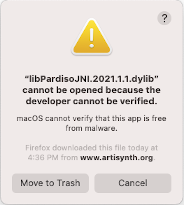
\includegraphics[]{images/MacSecurityNotice}
\else
  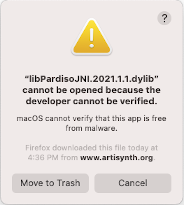
\includegraphics[width=2.5in]{images/MacSecurityNotice}
\fi
\end{center}
The problem here is that one or more of the native libraries are not ``known''
to Apple and are therefore not trusted. Clicking the "?" on the popup will
open a window containing more information about what to do.

The short version is to immediately open your Security and Privacy
settings after the error occurs, and then, near the bottom of the {\sf
General} tab, you should see a notification about the blocked
application with a button to the right labeled {\sf Open
Anyway}. Clicking that button will grant the application a security
exception. You will then need to exit and restart ArtiSynth.

\end{document}
